% 5
\chapter{バランス化推論システム}

%2024年9月7日木曜日から9月8日金曜日まで崇城大学にて行われた2023年度(第76回)電気・情報関係学会九州支部連合大会で口頭発表を行った内容である.

並列ランダムアクセス機械(Parallel Random Access Machine,PRAMと略す)とは,共有メモリをプロセッサ間の通信手段とする並列計算の理論的モデルである\cite{greenlaw-parallel1995, miyano-parallel1993}.効率のよい並列アルゴリズムとは,入力サイズ$n$に対して,$O(n^k)$個のプロセッサを持つPRAM上で,$O((\log n)^{c})$時間で計算するアルゴリズム(ただし$k$と$c$は$n$に依存しない定数)のことをいう.効率のよい並列アルゴリズムを持つ計算問題のクラスをNC(Nick's Class)という.クラスPに含まれる計算問題がいつでもNCに含まれるかという問いは並列計算量理論における未解決問題である.

財津\cite{zaitsu}は,推論システムのバランス化を用いて,線形順序項木パターンと順序木を入力とするパターン照合問題に対して,効率の良い並列アルゴリズムを提案した.しかし,そのアルゴリズムは,\cite{miyano-parallel1993}の補題8.1(p.246)の誤りにより正しい並列計算量が得られないことがわかった.そこで本章では,その誤りを訂正し(補題\ref{lem:base}),新しい推論規則とそれを用いる推論システムのバランス化を提案して,バランス化の理論的解析を行う.これにより得られた定理は,線形順序項木パターンと順序木を入力とするパターン照合問題,または子の数の最大値2の線形無順序項木パターンと無順序木を入力とするパターン照合問題への効率の良い並列アルゴリズムの設計に対する基盤となる.

% 5.1
\section{バランス化推論システム}
%本章では,無順序木と順序木に共通する性質を議論する.
以降,無順序木または順序木をまとめて根付き木とよぶ.根付き木$T$の頂点数および高さを,それぞれ$size(T)$および$height(T)$で表す.任意の根付き木$T$と$T$の頂点$v$に対して,$T(v)$は$v$のすべての子孫からなる$T$の部分木を表す.また,$\overline{T}(v)$は$v$の真の子孫を削除して得られる$T$の部分木を表す.

$X$を有限集合とする.本章では$X$の要素を\textbf{文(sentence)}とよぶことにする.
$n+1$個$(n\geq 0)$の文$\alpha,\beta_{1},\ldots,\beta_{n}\in X$に対して,
$\alpha \leftarrow \beta_{1}, \ldots, \beta_{n}$の形を\textbf{推論規則(inference rule)}とよぶ.
文の集合$X$と推論規則の集合$R$の二つ組$Q=(X,R)$を\textbf{推論システム(inference system)}とよぶ.
$\alpha \leftarrow$の形の推論規則があるとき,文$\alpha$を\textbf{公理(axiom)}とよぶ.

推論システム$Q=(X,R)$に対して,公理の集合を$\textbf{AXIOM}(Q)$と書く.
$\textbf{TH}(Q)$を,次の(1)から始めて,(2)を再帰的に用いて得られる$X$の部分集合とする.
\begin{enumerate}
\item[(1)] $\textbf{TH}(Q)=\textbf{AXIOM}(Q)$とする.
\item[(2)] $\beta_{1},\ldots,\beta_{n}\in \textbf{TH}(Q)$かつ
$\alpha \leftarrow \beta_{1}, \ldots, \beta_{n}\in R$ならば,$\alpha\in\textbf{TH}(Q)$とする.
\end{enumerate}

文$\gamma\in X$の$Q=(X,R)$における\textbf{証明木(proof tree)}とは,次の条件(1)--(3)を満たす無順序木$T$である.
\begin{enumerate}
\item 根のラベルは$\gamma$である.
\item 文$\alpha\in X$をラベルとする頂点が$k$個$(k\geq 1)$の子を持ち,そのラベルがそれぞれ$\beta_{1},\ldots,\beta_{k}$であれば, 推論規則$\alpha \leftarrow \beta_{1}, \ldots, \beta_{k}$が$R$の要素である.
\item 文$\alpha\in X$をラベルとする頂点が$T$の葉ならば,$\alpha\in \textbf{AXIOM}(Q)$である.
\end{enumerate}

上記の条件(1)--(3)のうち,(1)と(2)を満たす無順序木$T$を\textbf{推論木(inference tree)}とよぶ.$\gamma\in \textbf{TH}(Q)$に対して,$\gamma$を根のラベルとする証明木$T(\gamma)$は一般に存在する.このとき
  \begin{eqnarray*}
    && proof\mbox{-}tree_Q(\gamma)=\min\{size(T(\gamma))\mid T(\gamma)は\gamma の証明木\}\\
    && proof\mbox{-}tree(Q)=\max\{proof\mbox{-}size(\gamma)\mid \gamma\in \textbf{TH}(Q)\}
  \end{eqnarray*}
  と定義し,$proof$-$size(\gamma)$を$Q$における$\gamma$の証明サイズ(proof-size),$proof$-$size(Q)$を推論システム$Q$の証明サイズと呼ぶ.同様にして
  \begin{eqnarray*}
    && height_Q(\gamma)=\min\{height(T(\gamma))\mid T(\gamma)は\gamma の証明木\}\\
    && height(Q)=\max\{height(\gamma)\mid \gamma\in \textbf{TH}(Q)\}
  \end{eqnarray*}
  と定義する.

本研究では,\cite{miyano-parallel1993}で定義されたバランス化推論システムに新しく推論規則を導入して,正しいバランス化が行われる推論システムを構築した.具体的に本研究で提案した推論規則は,次の定義\ref{def5}の(c1), (c2), (e)である.

% 定義10
\begin{define}\label{def5}
推論システム$Q=(X,R)$に対して次のように定義される推論システム$Q^{B}=(X^{B},R^{B})$を$Q$の\textbf{バランス化推論システム(balanced inference system)}と呼ぶ.
\end{define}
\begin{enumerate}
  \item $X^{B}=X\cup(X\times X)\cup(X\times(X\times X))$.
  \item $R^{B}$は次のものからなる.
  \begin{enumerate}
    \item $R$の推論規則に対して,それぞれ$R^{B}$の推論規則を次のように定義する.
    \begin{table}[H]
    \centering
    \begin{tabular}{|c|c|}\hline
      $R$の推論規則 & $R^{B}$の推論規則 \\ \hline\hline
      $x\leftarrow$ & $x\leftarrow$ \\
      $x\leftarrow y$ & $(y,x)\leftarrow$ \\
      $x\leftarrow z,y$ & $(z,(y,x))\leftarrow$ \\
      $x\leftarrow z,y$ & $(y,(z,x))\leftarrow$ \\ \hline
    \end{tabular}
  \end{table}
    \item $x\leftarrow y,(y,x)$
    \item[(c1)] $(y,x)\leftarrow z,(z,(y,x))$
    \item[(c2)] $(z,x)\leftarrow y,(z,(y,x))$
    \item[(d)] $(z,x)\leftarrow (z,y),(y,x)$
    \item[(e)] $(z,(y,x))\leftarrow (z,w),(w,(y,x))$
  \end{enumerate}
\end{enumerate}

%バランス化推論システム$Q^{B}=(X^{B},R^{B})$の推論規則のうち$Q=(X,R)$の推論規則に依存するものは(a)で与えられるもののみで,(b)〜(d)の推論規則は$R$の構造に無関係であることに注意する.

\cite{miyano-parallel1993}より,次の命題が成立する.
\begin{proposition}
  推論システム$Q=(X,R)$とそのバランス化推論システム$Q^{B}=(X^{B},R^{B})$に対して
  \begin{eqnarray*}
    \textbf{TH}(Q)=\textbf{TH}(Q^{B})\cap X
  \end{eqnarray*}
  が成り立つ.
\end{proposition}

% 5.1.1
%\documentclass[11pt]{jsarticle}
%\usepackage{amsmath,amssymb}
%\usepackage[dvipdfmx]{graphicx}
%
%\pagestyle{plain}
%
%\newtheorem{theorem}{定理}
%\newtheorem{lemma}{補題}
%\newtheorem{proposition}{命題}
%\newtheorem{corollary}{系}
%\newtheorem{define}{定義}
%\newtheorem{example}{例}
%\newenvironment{proof}{\noindent{\bf 証明.}}{\hfill {$\Box$}\par\medskip}
%
%\begin{document}
%\section{バランス化推論システムの理論的解析}

% 5.1.2
\subsection{根付き2分木のバランス化}

%本章では,無順序木と順序木に共通する性質を議論する.以降,無順序木または順序木をまとめて根付き木とよぶ.根付き木$T$の頂点数および高さを,それぞれ$size(T)$および$height(T)$で表す.任意の根付き木$T$と$T$の頂点$v$に対して,$T(v)$は$v$のすべての子孫からなる$T$の部分木を表す.また,$\overline{T}(v)$は$v$の真の子孫を削除して得られる$T$の部分木を表す.

本項では,バランス化を行うために必要な命題と補題を証明する.

% 命題3
\begin{proposition}\label{prop:base}
任意の根付き木$T$には次の2つの条件を満たす頂点$u$が存在する.
\begin{enumerate}
  \item[(a)] $\displaystyle size(\overline{T}(u))\leq\left\lceil\frac{1}{3}size(T)\right\rceil$,
  \item[(b)] $u$が子$w$を持つならば,$\displaystyle size(\overline{T}(w))>\left\lceil\frac{1}{3}size(T)\right\rceil$.
\end{enumerate}
\end{proposition}

\begin{proof}
条件(a)を満たす頂点は必ず存在する.たとえば,$r$を$T$の根とすると,$size(\overline{T}(r))=1$であるから,条件(a)はいつでも成り立つ.
そこで,条件(a)を満たす頂点$u$に対して,次の操作を繰り返す:
$u$の子$w$で条件(b)が成り立たない頂点が存在すれば,$size(\overline{T}(w))\leq\left\lceil\frac{1}{3}size(T)\right\rceil$であるので,$w$は条件(a)を満たし,さらに$u$より深さが1だけ大きい.そこで,この$w$をあらためて$u$とる.
条件(a)を満たす$u$が葉であれば,すなわち$u$が子を持たないのであれば,条件(b)は成り立つ.よって,この操作を繰り返せば,深さは有限であるので,条件(a),(b)を満たす頂点$u$を得ることができる.
\end{proof}

\cite{miyano-parallel1993}の補題8.1(p.246)に誤りがある.その補題の代わりに本項では次の補題を示す.

% 命題4
\begin{proposition}\label{prop:int1}
$n\in \mathbb{Z}$に対して,次の等式が成り立つ.
$$
  \left\lceil\frac{n}{3}\right\rceil + \left\lfloor\frac{2 n}{3}\right\rfloor = n.
$$
\end{proposition}

\begin{proof}
  \begin{enumerate}
  \item $n = 3m$ ($m \in \mathbb{Z}$)のとき,
  $$\left\lceil\frac{3m}{3}\right\rceil + \left\lfloor\frac{2\cdot 3m}{3}\right\rfloor = m + 2m = 3 m = n.$$
  \item $n = 3m + \ell$ ($m \in \mathbb{Z}$, $\ell = 1,2$)のとき,
  $$\left\lceil\frac{km+\ell}{k}\right\rceil + \left\lfloor\frac{(k-1)(km+\ell)}{k}\right\rfloor = m + 1 + (k-1)m + \ell - 1 = k m + \ell = n.$$
  \end{enumerate}
  以上より,与式が成り立つ.
\end{proof}

% 命題5
\begin{proposition}\label{prop:int2}
  $n\in \mathbb{Z}$に対して,次の不等式が成り立つ.
  $$
  \left\lceil\frac{2n}{3}\right\rceil \geq
  n - \left\lceil\frac{2n}{3}\right\rceil + \left\lceil\frac{n}{3}\right\rceil.
  $$
\end{proposition}
  
\begin{proof}
  \begin{enumerate}
    \item $n = 3m$ ($m \in \mathbb{Z}$)のとき,
    \begin{align*}
    \mbox{左辺} & = \left\lceil\frac{6 m}{3}\right\rceil = 2m,\\
    \mbox{右辺} & = 3 m - \left\lceil\frac{6 m}{3}\right\rceil + \left\lceil\frac{3 m}{3}\right\rceil = 3m - 2m + m = 2m.
    \end{align*}
    \item $n = 3m + 1$ ($m \in \mathbb{Z}$)のとき,
    \begin{align*}
    \mbox{左辺} & = \left\lceil\frac{2(3 m + 1)}{3}\right\rceil = 2m + 1,\\
    \mbox{右辺} & = 3 m + 1 - \left\lceil\frac{2(3 m + 1)}{3}\right\rceil + \left\lceil\frac{3 m + 1}{3}\right\rceil
    = 3 m + 1 - (2m + 1) + m + 1 = 2m + 1.
    \end{align*}
    \item $n = 3m + 2$ ($m \in \mathbb{Z}$)のとき,
    \begin{align*}
    \mbox{左辺} & = \left\lceil\frac{2(3 m + 2)}{3}\right\rceil = 2m + 2,\\
    \mbox{右辺} & = 3 m + 2 - \left\lceil\frac{2(3 m + 2)}{3}\right\rceil + \left\lceil\frac{3 m + 2}{3}\right\rceil
    = 3 m + 2 - (2m + 2) + m + 1 = 2m + 1.
    \end{align*}
  \end{enumerate}
  以上より,いずれの場合も$\mbox{左辺}\geq\mbox{右辺}$が成り立つ.
\end{proof}

% 補題4
\begin{lemma}\label{lem:base}
  任意の根付き2分木$T$には次の2つの条件を満たす頂点$v$が存在する.
  \begin{enumerate}
    \item[(1)] $\displaystyle size(T(v))\leq\left\lceil\frac{2}{3}size(T)\right\rceil$,\smallskip
    \item[(2)] $\displaystyle size(\overline{T}(v))\leq\left\lceil\frac{2}{3}size(T)\right\rceil + 1$.
  \end{enumerate}
\end{lemma}

\begin{proof}
  $T$には命題\ref{prop:base}の条件(a),(b)を満たす頂点$u$が存在する.
  \begin{enumerate}
  \item $u$が子を持たないとき($u$が葉のとき): $\overline{T}(u)=T$であるから,命題\ref{prop:base}の条件(a)より,
$$size(T)\leq\left\lceil\frac{1}{3}size(T)\right\rceil$$となる.これより$size(T)=1$が得られる.すなわち,$u$は$T$の唯一の頂点であり,この$u$を$v$とすることで,条件(1),(2)を満たす.

\item $u$が1つの子$w$を持つとき:
$w$が条件(1),(2)の$v$になることを示す.
命題\ref{prop:base}の条件(b)より,
$$size(\overline{T}(w))>\left\lceil\frac{1}{3}size(T)\right\rceil.$$
$size(T(w)) + size(\overline{T}(w)) = size(T) + 1$より,
$$size(T(w)) = size(T) - size(\overline{T}(w)) + 1
< size(T) - \left\lceil\frac{1}{3}size(T)\right\rceil + 1.$$
この不等式はすべて整数の項から成るので,次の不等式が得られる.
$$size(T(w)) \leq size(T) - \left\lceil\frac{1}{3}size(T)\right\rceil.$$
命題\ref{prop:int1}より,
$$size(T(w)) \leq \left\lfloor\frac{2}{3}size(T)\right\rfloor
\leq\left\lceil\frac{2}{3}size(T)\right\rceil.$$
以上より,$w$が条件(1)を満たすことが示された.次に$w$に対して,
条件(2)が成り立たないとして矛盾を導く.具体的には,次の不等式(i)が成り立つと仮定する.
\begin{align*}
size(\overline{T}(w))&>\left\lceil\frac{2}{3}size(T)\right\rceil + 1.\tag{i}
\end{align*}
$size(T(w)) + size(\overline{T}(w)) = size(T) + 1$と不等式(i)より,
\begin{align*}
size(T(w)) = size(T) + 1 - size(\overline{T}(w)) < size(T) - \left\lceil\frac{2}{3}size(T)\right\rceil.\tag{ii}
\end{align*}
したがって,不等式(i)と(ii),命題\ref{prop:base}の条件(a)より,
$$
\left\lceil\frac{2}{3}size(T)\right\rceil < size(\overline{T}(w_{1})) - 1
  = (size(\overline{T}(u)) + 1) - 1
  = size(\overline{T}(u))
  < \left\lceil\frac{1}{3}size(T)\right\rceil.
$$
これは自然数の大小関係に矛盾する.以上より,$w$が条件(2)も満たすことが示された.

\item $u$が2つの子$w_{1},w_{2}$を持つとき: $size(T(w_{1}))\geq size(T(w_{2}))$として一般性を失わない.
$w_{1}$が条件(1),(2)の$v$になることを示す.
命題\ref{prop:base}の条件(b)より,
$$size(\overline{T}(w_{1}))>\left\lceil\frac{1}{3}size(T)\right\rceil.$$
$size(T(w_{1})) + size(\overline{T}(w_{1})) = size(T) + 1$より,
$$size(T(w_{1})) = size(T) - size(\overline{T}(w_{1})) + 1
< size(T) - \left\lceil\frac{1}{3}size(T)\right\rceil + 1.$$
この不等式はすべて整数の項から成るので,次の不等式が得られる.
$$size(T(w_{1})) \leq size(T) - \left\lceil\frac{1}{3}size(T)\right\rceil.$$
命題\ref{prop:int1}より,
$$size(T(w_{1})) \leq \left\lfloor\frac{2}{3}size(T)\right\rfloor
\leq\left\lceil\frac{2}{3}size(T)\right\rceil.$$
以上より,$w_{1}$が条件(1)を満たすことが示された.次に$w_{1}$に対して,
条件(2)が成り立たないとして矛盾を導く.具体的には,次の不等式(iii)が成り立つと仮定する.
\begin{align*}
size(\overline{T}(w_{1}))&>\left\lceil\frac{2}{3}size(T)\right\rceil + 1.\tag{iii}
\end{align*}
$size(T(w_{1})) + size(\overline{T}(w_{1})) = size(T) + 1$と不等式(iii)より,
\begin{align*}
size(T(w_{1})) = size(T) + 1 - size(\overline{T}(w_{1})) < size(T) - \left\lceil\frac{2}{3}size(T)\right\rceil.
\end{align*}
$size(T(w_{1}))\geq size(T(w_{2}))$としたので,次の不等式が得られる.
\begin{align*}
size(T(w_{2})) < size(T) - \left\lceil\frac{2}{3}size(T)\right\rceil.\tag{iv}
\end{align*}
したがって,不等式(iii)と(iv),命題\ref{prop:base}の条件(a)より,
\begin{align*}
  \left\lceil\frac{2}{3}size(T)\right\rceil & < size(\overline{T}(w_{1})) - 1\\
  & = (size(T(w_{2})) + size(\overline{T}(u)) + 1) - 1\\
  & = size(T(w_{2})) + size(\overline{T}(u))\\
  & < size(T) - \left\lceil\frac{2}{3}size(T)\right\rceil + \left\lceil\frac{1}{3}size(T)\right\rceil
  \end{align*}
これは命題\ref{prop:int2}に矛盾する.以上より,$w_{1}$が条件(2)も満たすことが示された.
\end{enumerate}
\end{proof}

% 命題6
\begin{proposition}\label{prop:int3}
$n\in\mathbb{N}$に対して,$n\geq 18$のとき,次の不等式が成り立つ.
$$
\left\lceil\frac{2}{3}n\right\rceil + 1 \leq \frac{3}{4}n.
$$
\end{proposition}
\begin{proof}
$\displaystyle S = \frac{3}{4}n - \left\lceil\frac{2}{3}n\right\rceil - 1$とおく.
\begin{enumerate}
\item $n = 12 m + 3 m^{\prime}$ $(m, m^{\prime} \in \mathbb{Z}, 0\leq m^{\prime} \leq 3)$のとき,
$$S = \frac{3}{4}(12 m + 3 m^{\prime}) - \left\lceil\frac{2}{3}(12 m + 3 m^{\prime})\right\rceil - 1
 = m + \frac{1}{4}m^{\prime} - 1.$$
したがって,$m\geq 1, 0\leq m^{\prime} \leq 3$のとき,$S \geq 0$である.
\item $n = 12 m + 3 m^{\prime} + 1$ $(m, m^{\prime} \in \mathbb{Z}, 0\leq m^{\prime} \leq 3)$のとき,
$$S = \frac{3}{4}(12 m + 3 m^{\prime} + 1) - \left\lceil\frac{2}{3}(12 m + 3 m^{\prime} + 1)\right\rceil - 1
 = m + \frac{1}{4}m^{\prime} - \frac{5}{4}.$$
したがって,$(m,m^{\prime}) = (1, 1), (1, 2), (1, 3)$ 及び $m \geq 2, 0\leq m^{\prime} \leq 3$のとき,$S \geq 0$である.
\item $n = 12 m + 3 m^{\prime} + 2$ $(m, m^{\prime} \in \mathbb{Z}, 0\leq m^{\prime} \leq 3)$のとき,
$$S = \frac{3}{4}(12 m + 3 m^{\prime} + 2) - \left\lceil\frac{2}{3}(12 m + 3 m^{\prime} + 2)\right\rceil - 1
 = m + \frac{1}{4}m^{\prime} - \frac{3}{2}.$$
したがって,$(m,m^{\prime}) = (1, 2), (1, 3)$ 及び $m \geq 2, 0\leq m^{\prime} \leq 3$のとき,$S \geq 0$である.
\end{enumerate}
以上より,$n\geq 18$のとき$S > 0$となる.したがって本命題が成り立つ.
\end{proof}

% 系1
\begin{corollary}\label{cor:1}
  根付き2分木$T$が$size(T)\geq 18$であるとき,$T$には次の2つの条件を満たす頂点$v$が存在する.
  \begin{enumerate}
  \item[(1)] $\displaystyle size(T(v)) < \frac{3}{4}size(T)$,\smallskip
  \item[(2)] $\displaystyle size(\overline{T}(v)) < \frac{3}{4}size(T)$.
  \end{enumerate}
\end{corollary}

\begin{proof}
補題\ref{lem:base}と命題\ref{prop:int3}から示される.
\end{proof}

% 5.1.2
\subsection{バランス化推論システムの高さに関する定理}
% 命題7
\begin{proposition}\label{prop:main}
  $a \geq 2$ $(a\in\mathbb{N})$に対して,$H:\mathbb{N}\rightarrow \mathbb{R}$を次の性質を持つ関数とする.
$$H(n) \leq 
\begin{cases}
n & (1\leq n \leq 17),\\
H(\frac{3}{4}n) + a & (n\geq 18).
\end{cases}
$$
  このとき,$n\geq 18$に対して,次の不等式が成り立つ.
  $$
  H(n) < \frac{a}{\log_{2}\frac{4}{3}} \log_{2} n.
  $$
\end{proposition}

\begin{proof}
$\ell \in \mathbb{N}$に対して,
$$
H(n) \leq H\left(\left(\frac{3}{4}\right)^{\ell}n\right) + \ell\cdot a
$$
が成り立つ.$\left(\frac{3}{4}\right)^{\ell}n\leq 17$を$\ell$に関して解くと,
$\displaystyle\ell\geq \frac{\log_{2}n - \log_{2}17}{\log_{2}\frac{4}{3}}$を得る.
したがって,$\log_{2}17 \leq 4.0875$であること,さらに$a\geq 2$に対して,$\displaystyle\frac{a\log_{2}17}{\log_{2}\frac{4}{3}} > 19$であることから,
\begin{align*}
H(n) & \leq 17 + \frac{\log_{2}n - \log_{2}17}{\log_{2}\frac{4}{3}}\cdot a
 = \frac{a}{\log_{2}\frac{4}{3}}\log_{2}n + 17 - \frac{a\log_{2}17}{\log_{2}\frac{4}{3}} < \frac{a}{\log_{2}\frac{4}{3}} \log_{2} n
\end{align*}
が得られる.
\end{proof}

% 系2
\begin{corollary}\label{cor:2}
  $H:\mathbb{N}\rightarrow \mathbb{R}$を次の性質を持つ関数とする.
$$H(n) \leq 
\begin{cases}
n & (1\leq n \leq 17),\\
H(\frac{3}{4}n) + 3 & (n\geq 18).
\end{cases}
$$
このとき,次の不等式が成り立つ.
$$H(n) \leq 
\begin{cases}
1 & (n = 1),\\
7 \log_{2}n & (n\geq 2).
\end{cases}
$$
\end{corollary}

\begin{proof}
$0.4150 < \log_{2}\frac{4}{3} < 0.4151$であること,
$2\leq n\leq 17$に対して$n \leq 7\log_{2}n$であることから,命題\ref{prop:main}より本系が得られる.
\end{proof}

%%%%%
% もっと係数が小さくならないか試しに計算してみただけなので削除して良いです.
% 考察内の$k$を大きくすれば,係数は小さくなると思います.
% ただし,その係数を持つ$H(n)$の評価を満たす$n$が$k^2$に比例して大きくなります.
% したがって,あまりメリットはないと結論しました.
%%%%
\if0
\subsection*{考察}

\begin{proposition}\label{prop:int4}
  $n, k\in\mathbb{N}$に対して,$n\geq 3k(2k + 1)$のとき,次の不等式が成り立つ.
  $$
  \left\lceil\frac{2}{3}n\right\rceil + 1 < \frac{2k+1}{3k}n.
  $$
  \end{proposition}
  \begin{proof}
  $\displaystyle S = \frac{2k+1}{3k}n - \left\lceil\frac{2}{3}n\right\rceil - 1$とおく.
  $n = 3k m + \ell$ $(m \in \mathbb{Z}, 0\leq \ell < 3k)$のとき,
  \begin{align*}
  S & = \frac{2k + 1}{3k}(3k m + \ell) - \left\lceil\frac{2}{3}(3k m + \ell)\right\rceil - 1\\
  & = (2k + 1)m + \frac{2k + 1}{3k}\cdot\ell - (2k m + \left\lceil\frac{2}{3}\ell\right\rceil) - 1\\
  &= m + \frac{2k + 1}{3k}\cdot\ell - \left\lceil\frac{2}{3}\ell\right\rceil - 1\\
  &\geq m + \frac{2k + 1}{3k}\cdot\ell - \left\lceil\frac{2}{3}(3k - 1)\right\rceil - 1\\
  &\geq m + \frac{2k + 1}{3k}\cdot\ell - 2k - 1\\
  &= m - \frac{(2k + 1)(3k - \ell)}{3k}\\
  &\geq m - (2k + 1).
  \end{align*}
  したがって,$m\geq 2k + 1$のとき,$S \geq 0$である.
  以上より,$n\geq 3k(2k + 1)$のとき,本命題が成り立つ.$k=2$のとき,$n\geq 30$である.
  \end{proof}
\fi
%%%%
%\end{document}

%5.1.3
\subsection{バランス化推論システムによる高さの抑制}
本項では,提案したバランス化推論システムによる高さの抑制について述べる.証明の流れは\cite{miyano-parallel1993}と同じである.
$Q=(X,R)$のバランス化推論システム$Q^{B}=(X^{B},R^{B})$に文の個数は$|X^{B}|=|X|+|X|^2+|X|^3$である.また$|R|\leq |X|+|X|^2+|X|^3$であるので,$Q^{B}$の推論規則の個数は$|R^{B}|=|R|+|X|^2+3|X|^3+|X|^4\leq |X|+2|X|^2+4|X|^3+|X|^4$という関係を満たす.したがって$Q^B$のサイズは$Q$のサイズの多項式である.次の定理が本章の主定理である.

% 定理2
\begin{theorem}\label{prop:int0}
  推論システム$Q$の任意の定理$\gamma$に対して,
  \begin{eqnarray*}
    height_{Q^{B}}(\gamma)\leq 7\cdot \log(\mbox{proof-size}_{Q}(\gamma))
  \end{eqnarray*}
  が成り立つ.
\end{theorem}

  %図5.1
  \begin{figure}[tb]
    \centering
    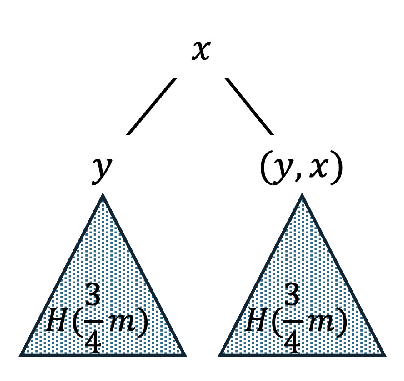
\includegraphics[scale=0.8]{fig-x_proof_tree.eps}
    \caption{$Q^{B}$における$x$の証明木で高さは,高々$H(\frac{3}{4}m)+1$である.}\label{fig-x_proof_tree}
    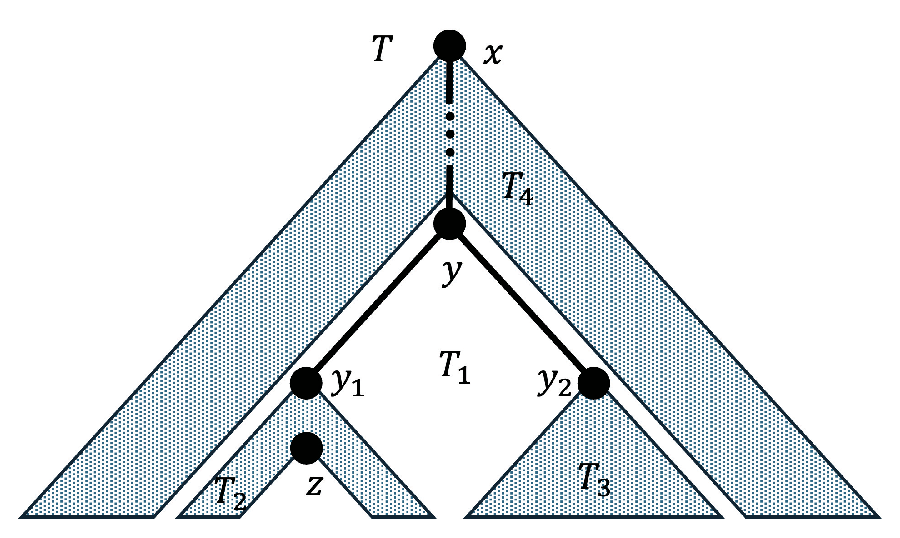
\includegraphics[scale=0.7]{fig-sub_proof_tree.eps}
    \caption{$Q$における仮定$z$での$x$の部分証明木}\label{fig:sub_proof_tree}
  \end{figure}

% 図5.2
\begin{figure}[tb]
  \centering
  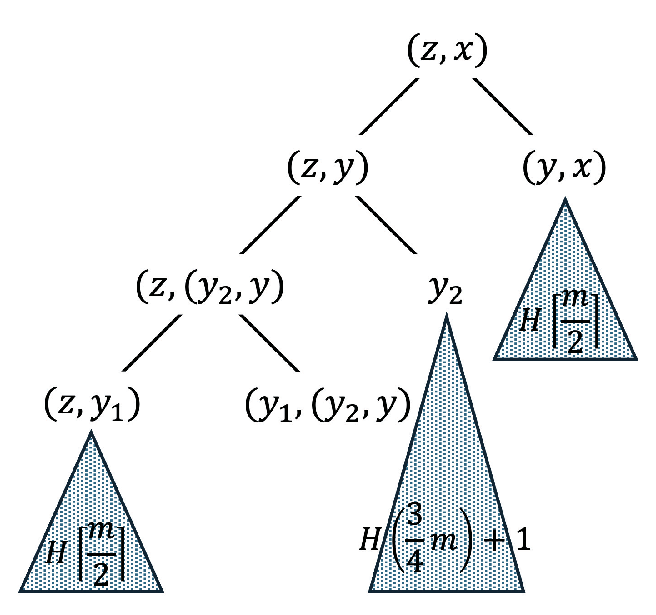
\includegraphics[scale=0.66]{fig-proof_tree.eps}
  \caption{$Q^{B}$における$(z,x)$の証明木}\label{fig:proof_tree}
\end{figure}

% 追加
\begin{proof}%[\textbf{命題\ref{prop:int0}の証明}]
  %$Q$における定理$\gamma$の証明木$T(\gamma)$に対して
  %$$height(T^{B}(\gamma))\leq 7\cdot \log(size(T(\gamma)))$$
  %を満たすバランス化推論システム$Q^{B}$における$\gamma$の証明木$T^{B}(\gamma)$が存在することを示せばよい.

  $x,y\in X$を$x\neq y$である$Q$の文とする.$Q$における仮定$y$のもとでの$x$の部分証明木とは,その根のラベルが$x$で,葉の中の1つのラベルが$y$でその他のラベルはすべて$Q$の公理であるような$Q$の推論木である.正整数$m\geq1$に対して,$S_1(m),S_2(m),H(m)$を次のように定義する.

    $S_1(m)=\{x\in X\mid Qにおけるサイズが高々mのxの証明木がある\}$,

    $S_2(m)=\{(y,x)\in X\times X\mid Qにおけるサイズが高々mの仮定yのもとでのxの部分証明木がある\}$,

    $H(m)=\max\{height_{Q^{B}}(\alpha)\mid\alpha\in S_1(m)\cup S_2(m)\}$.

  %$Q$においてサイズが1の証明木をもつものは,$Q$の公理だけであり,その証明木は根だけからなる高さが0の木である.また$S_2(1)$は空集合である.したがって$H(1)=0$である.また,$Q$においてサイズが2の証明木および仮定のもとでの部分証明木は$R$の推論規則$x\leftarrow y$から得られるものであり,このとき$(x,y)$は$Q^{B}$の公理である.したがって$H(2)=0$である.

  $m\leq 17$のとき,明らかに$H(m)\leq m$である.$m\geq 18$とし,$1\leq k\leq m-1$について$H(k)$が定まっているとする.$H(m)$に関して,次の場合を考える.
\begin{enumerate}
  \item $x\in S_1(m)$:このときサイズが高々$m$の$Q$における$x$の証明木$T$がある.系\ref{cor:1}より,$T$の頂点$y$で,$y$を根とする$T$の部分木を$T_1$とし,$T$から$T_1$の根以外の$T_1$の部分を取り除いた部分木を$T_2$とするとき,
  $$size(T_1)\leq\frac{3}{4}m, ~size(T_2)\leq\frac{3}{4}m$$
  となるものが存在する.よって,$y\in S_1(\frac{3}{4}m),(y,x)\in S_2(\frac{3}{4}m)$である.$m\geq18$のとき$m-1\geq\frac{3}{4}m$であることから$H(\frac{3}{4}m)$は定まっている.$Q^{B}$の推論規則$x\leftarrow y,(y,x)$を使い,$Q^{B}$における$x$の証明木で高さが高々$H(\frac{3}{4}m)+1$のものを構成できる(図\ref{fig-x_proof_tree}).したがって,次が成り立つ.
  $$H(m)\leq H(\frac{3}{4}m)+1$$

  \item $(z,x)\in S_2(m)$:このときサイズが高々$m$の$Q$における仮定$z$をのもとでの$x$の部分証明木$T$がある.そこで$T$の葉$z$から根$x$へ到達する道を$z$から$x$へたどっていくとき$size(T_1)>\left\lceil{\frac{size(T)}{2}}\right\rceil$となる初めての頂点を$y$とする.$T_1$を$y$を根とする$T$の部分木とする.頂点$y$の子で$y$と$z$を結ぶ道上にある頂点を$y_1$とするとき,葉$z$を含み頂点$y_1$を根とする部分木を$T_2$とする.$y$に$y_1$以外の子$y_2$があるときは,$y_2$を根とする部分木を$T_3$とする,$T_4$は$T$から$T_1$を取り除いた部分木とする(図\ref{fig:sub_proof_tree}).このとき,次の式が成り立つ.
  $$size(T_4)\leq\left\lceil{\frac{1}{2}m}\right\rceil,size(T_2)\leq\left\lceil{\frac{1}{2}m}\right\rceil, size(T_3)\leq m.$$
  図\ref{fig:proof_tree}の証明木を構成することで,$Q^{B}$における$(z,x)$の証明木ができる.したがって,次の式が成り立つ.
  $$H(m)\leq H(\frac{3}{4}m)+3.$$
\end{enumerate}

  以上の1と2から,$H(m)\leq m$ $(m\leq 17)$, $H(m)\leq H(\frac{3}{4}m)+3$ $(m\geq 18)$となり,系2より,$m=1$のとき$H(m)=1$,$m\geq 2$のとき$H(m)\leq 7\log m$が成り立つ.
\end{proof}

% 5.2
%\section{バランス化推論システムの実験的評価と今後の課題}
%最初に,二分化された順序木に対する均衡化について述べる.ページ数の都合上,二分線形順序項木パターンに対する均衡化の詳細は省略する.順序木$T=(V_T,E_T)$を変数集合が空である線形順序項木パターンとみなし,
二分化を行った順序木\cite{miyano-parallel1993}または子の数の最大値2の無順序木を,その構造の情報を保ったままバランス化が可能である.
%を$B(T)$とする.次のように$B(T)$を均衡化する.二分均衡化された$B(T)$の任意の頂点は高々2頂点を子として持つ.最初に,$B(T)$の頂点の頂点識別子$\alpha_0$とその子の頂点識別子 $\alpha_1,\alpha_2$の関係を「公理」とみなす.
%\begin{eqnarray*}
%  S_0&=&\{\alpha_0\mid\alpha は子を持たない\},\\
%  S_1&=&\{(\alpha_1,\alpha_0)\mid\alpha_0は唯一つの子\alpha_1を持つ\},\\
%  S_2&=&\{(\alpha_2,(\alpha_1,\alpha_0)),(\alpha_1,(\alpha_2,\alpha_0))\mid\alpha_0は2つの子\alpha_1と\alpha_2を持つ\}
%\end{eqnarray*}
%$S=S_0\cup S_1\cup S_2$として,これを$B(T)$の公理集合と呼ぶ.頂点数$N$の順序木$T$に対して,$B(T)$の頂点数が2$N-1$であることから,$\abs{S}\leq 4N$である.この公理の集合に対して,次の3つの推論規則を用いて,$B(T)$の根の頂点識別子($T$の根の頂点識別子でもある)に対する証明木を構築する.
%\begin{eqnarray*}
%  x&\leftarrow&y,(y,x)\\
%  (y,x)&\leftarrow&z,(z,(y,x))\\
%  (z,x)&\leftarrow&(z,y),(y,x)
%\end{eqnarray*}
%本研究では更に以下の証明木を提案する.
%\begin{eqnarray*}
%  (z,(y,x))&\leftarrow&(z,w),(w,(y,x))\\
%  (z,x)&\leftarrow&y,(z,(y,x))
%\end{eqnarray*}
%
%頂点数$N$の順序木$T$に対する$B(T)$の証明木を,$N$の多項式サイズのプロセッサを持つPRAMにより$O(\log N)$時間で計算できることが,宮野\cite{miyano-parallel1993}のテキストp.252により示されている.また,同テキストp.246の命題8.2の証明を訂正することにより,頂点数$N$が6以上の順序木$T$に対して,高さが高々5$\log N$であるような証明木を構築できることが示される.高さが高々5$\log N$である$B(T)$の証明木のひとつを$B(T)^Q$とする.
$\log m$の係数7は理論的解析により得られたもので,実際には,図\ref{fig:binary}のように頂点数18以下の全ての順序木に対して,高さが高々2$\log m$の証明木が存在する.$m\geq 18$のとき,$\log m$の係数を理論的に7未満にできるか否かは未解決である.

%次に,動的計画法を用いて,$B(T)^Q$の各頂点$x$の深さの降順に,頂点$x$に対応可能な$B(t)$の証明木の頂点の集合(CS($x$)と記す)を決定する.より具体的には,$B(T)^Q$の各頂点$x$に対して,二分線形順序項木パターン$B(t)$の公理集合と上記の推論規則,さらに変数に依存した継承規則を用いて,あらかじめ計算された$x$の高々2つの子$y,z$のCS($y$)とCS($z$)からCS($x$)を決定する.$B(T)^Q$の同じ深さの頂点$x$に対しては並列にCS($x$)を計算できるので,計算時間は$B(T)^Q$の高さに依存する.以上より,次の定理を得る.証明は省略する.

% 図5.3
\begin{figure}[tb]
  \centering
  \includegraphics[scale=0.7]{binary.eps}
  \caption{頂点数とバランス化後の木の高さの解析}\label{fig:binary}
\end{figure}

% 5.3
%\section{今後の課題}
%並列ランダムアクセス機械(Parallel Random Access Machine,PRAMと略す)とは,共有メモリをプロセッサ間の通信手段とする並列計算の理論的モデルである\cite{greenlaw-parallel1995}\cite{miyano-parallel1993}.効率のよい並列アルゴリズムとは,入力サイズ$n$に対して,$O(n^k)$個のプロセッサを持つPRAM上で,$O((\log n)^{c})$時間で計算するアルゴリズム(ただし$k$と$c$は$n$に依存しない定数)のことをいう.効率のよい並列アルゴリズムを持つ計算問題のクラスをNC(Nick's Class)という.クラスPに含まれる計算問題がいつでもNCに含まれるかという問いは並列計算量理論における未解決問題である.財津[4]は,推論システムのバランス化を用いて,線形順序項木パターンと順序木を入力とするパターン照合問題に対して,効率の良い並列アルゴリズムを提案した.しかし,そのアルゴリズムは,\cite{miyano-parallel1993}の補題8.1(p.246)の誤りにより正しい並列計算量が得られない.そこで本章では,新しい推論規則とそれを用いる推論システムのバランス化を提案して,線形順序項木パターンと順序木,または子の数の最大値2の線形無順序項木パターンと無順序木を入力とするパターン照合問題の効率の良い並列アルゴリズムの設計と解析に対する基盤とする.

%の二分バランス化手法を提案した.本論文では,同テキスト\cite{miyano-parallel1993}中に示された推論の並列化手法の高さの見積りに関する証明の誤りを訂正た.
%し,実際に,頂点数$n$の線形順序項木パターンと頂点数$N$の順序木を,それぞれ高さ$O(\log n)$の線形順序項木パターンと高さ$O(\log N)$の順序木に変換できることを示す.さらに,線形順序項木パターン照合問題に対する並列アルゴリズム提案し,その並列アルゴリズムがPRAM上で,頂点数$n$の線形順序項木パターンと頂点数$N$の順序木に対して,$n$と$N$の多項式個のプロセッサを用いて,$O(\log n)$時間で解くことができることを示す.

%\section{二分線形順序項木パターン(今後の課題に)}
%$t=(V_t,E_t,H_t)$を線形順序項木パターンとする.以下では,$t$の頂点には,その頂点を識別する固有の番号または記号(列)が与えられているものとする.その番号を頂点識別子と呼び,$u\in V_t$に対して,$\langle u\rangle$で表す.同様に,$t$の辺と変数にも,それぞれ互いに異なる辺識別子と変数識別子が与えられており,各$(u_0,u_1)\in E_t$と$[u_0,u_1]\in E_t$に対して,同じ記号$\langle u_0,u_1 \rangle$で表す.$t$の任意の頂点$u_0$の子を兄弟の順に$u_1,u_2,\ldots,u_\ell(\ell\geq 0)$とし,$u_0$に対して,
%\begin{eqnarray*}
%  V_{B(t)}^{n_0}&=&\{\langle u_0\rangle,\langle u_1\rangle,\ldots,\langle u_\ell\rangle\}\cup\{\langle u_0,u_1\rangle,\ldots,\langle u_0,u_\ell\rangle\},\\
%  H_{B(t)}^{n_0}&=&\{(\langle u_0\rangle,\langle u_0,u_\ell\rangle),(\langle u_0,u_\ell\rangle,\langle u_\ell\rangle),(\langle u_0,u_\ell\rangle,\langle u_0,u_{\ell-1}\rangle)\mid[u_0,u_\ell]\in H_T\}\\
%  &\cup&\{(\langle u_0,u_{i+1}\rangle,\langle u_0,u_i\rangle),(\langle u_0,u_i\rangle,\langle u_i\rangle),(\langle u_0,u_i\rangle,\langle u_0,u_{i-1}\rangle)\mid[u_0,u_i]\in H_T,1<i<\ell\}\\
%  &\cup&\{(\langle u_0,u_2\rangle,\langle u_0,u_1\rangle),(\langle u_0,u_1\rangle,\langle u_1\rangle)\mid[u_0,u_1]\in H_T\},\\
%  E_{B(t)}^{n_0}&=&\{(\langle u_0\rangle,\langle u_0,u_\ell\rangle),(\langle u_0,u_i\rangle,\langle u_i\rangle),(\langle u_0,u_{i+1}\rangle,\langle u_0,u_i\rangle)\mid1\leq i\leq\ell\}\setminus H_{B(t)}^{u_0}
%\end{eqnarray*}
%とおく.$t$の二分線形順序項木パターンを
%\begin{eqnarray*}
%  B(t)=(\bigcup_{u_0\in V_t}V_{B(t)}^{u_0},\bigcup_{u_0\in V_t}E_{B(t)}^{u_0},\bigcup_{u_0\in V_t}H_{B(t)}^{u_0})
%\end{eqnarray*}
%とする.$B(t)$の頂点識別子で表される頂点$\langle u\rangle$を実頂点,辺識別子と変数識別子で表される頂点$\langle u,u'\rangle$を仮頂点と呼ぶ.図2に線形順序項木パターン$t$と二分線形順序項木パターン$B(t)$の例を示す.$n$頂点の線形順序項木パターン$t$に対して,二分線形順序項木パターン$B(t)$の頂点数は$2n-1$となる.